\chapter{Results}
\label{ch:Results}
We show the results of the different experiments and discuss their implications.

\section{Hyperparameter Search}
We list the selected learning rate and regularization parameter for the five folds of each experiment (Tab~\ref{tab:HSResults}).

\begin{table}[h]
	\centering
	\setlength\tabcolsep{3.5pt}
	\begin{tabular}{l*{10}{c}}
		\hline
		 & \multicolumn{2}{c}{\textbf{Fold 1}} & \multicolumn{2}{c}{\textbf{Fold 2}} &\multicolumn{2}{c}{\textbf{Fold 3}} &\multicolumn{2}{c}{\textbf{Fold 4}} &\multicolumn{2}{c}{\textbf{Fold 5}}\\
		& \textbf{$\alpha$} & \textbf{$\lambda$} & \textbf{$\alpha$} & \textbf{$\lambda$} & \textbf{$\alpha$} & \textbf{$\lambda$} & \textbf{$\alpha$} & \textbf{$\lambda$} & \textbf{$\alpha$} & \textbf{$\lambda$}\\
		\hline 
		Exp. 1.1	&\sn{2}{-4}	&\sn{3}{-2}	&\sn{2}{-4}	&\sn{4}{-2}	&\sn{9}{-5}	&\sn{5}{-3}	&\sn{6}{-4}	&\sn{8}{-3}	&\sn{6}{-4}	&\sn{1}{-2}\\
		Exp. 1.2	&\sn{4}{-4}	&\sn{9}{-2}	&\sn{4}{-4}	&\sn{5}{-2}	&\sn{4}{-4}	&\sn{7}{-3}	&\sn{3}{-4}	&\sn{5}{-3}	&\sn{6}{-4}	&\sn{3}{-2}\\
		Exp. 1.3	&\sn{4}{-4}	&\sn{3}{-2}	&\sn{2}{-4}	&\sn{4}{-2}	&\sn{7}{-5}	&\sn{6}{-3}	&\sn{4}{-4}	&\sn{8}{-2}	&\sn{8}{-4}	&\sn{3}{-2}\\
		Exp. 2		&\sn{1}{-5}	&\sn{4}{-4}	&\sn{5}{-5}	&\sn{4}{-3}	&\sn{5}{-5}	&\sn{1}{-3}	&\sn{1}{-5}	&\sn{2}{-4}	&\sn{5}{-5}	&\sn{2}{-4}\\
		Exp. 3		&\sn{1}{-4}	&\sn{4}{-4}	&\sn{7}{-5}	&\sn{5}{-4}	&\sn{1}{-4}	&\sn{7}{-4}	&\sn{7}{-5}	&\sn{2}{-4}	&\sn{8}{-5}	&\sn{9}{-5}\\
		\hline
	\end{tabular}
	\caption[Hyperparameter search results]{Selected learning rate and regularization parameter configurations.}
	\label{tab:HSResults}
\end{table}
% Discussion: Lambda is not as important as alpha. Highest alpha causes divergence, highest lambda causes convergence to a single point. In general, not so important.

\section{Experiments}
We show the FROC curves for each experiment and fold (Fig.~\ref{fig:FROCResults}).
\begin{figure}
	\centering
		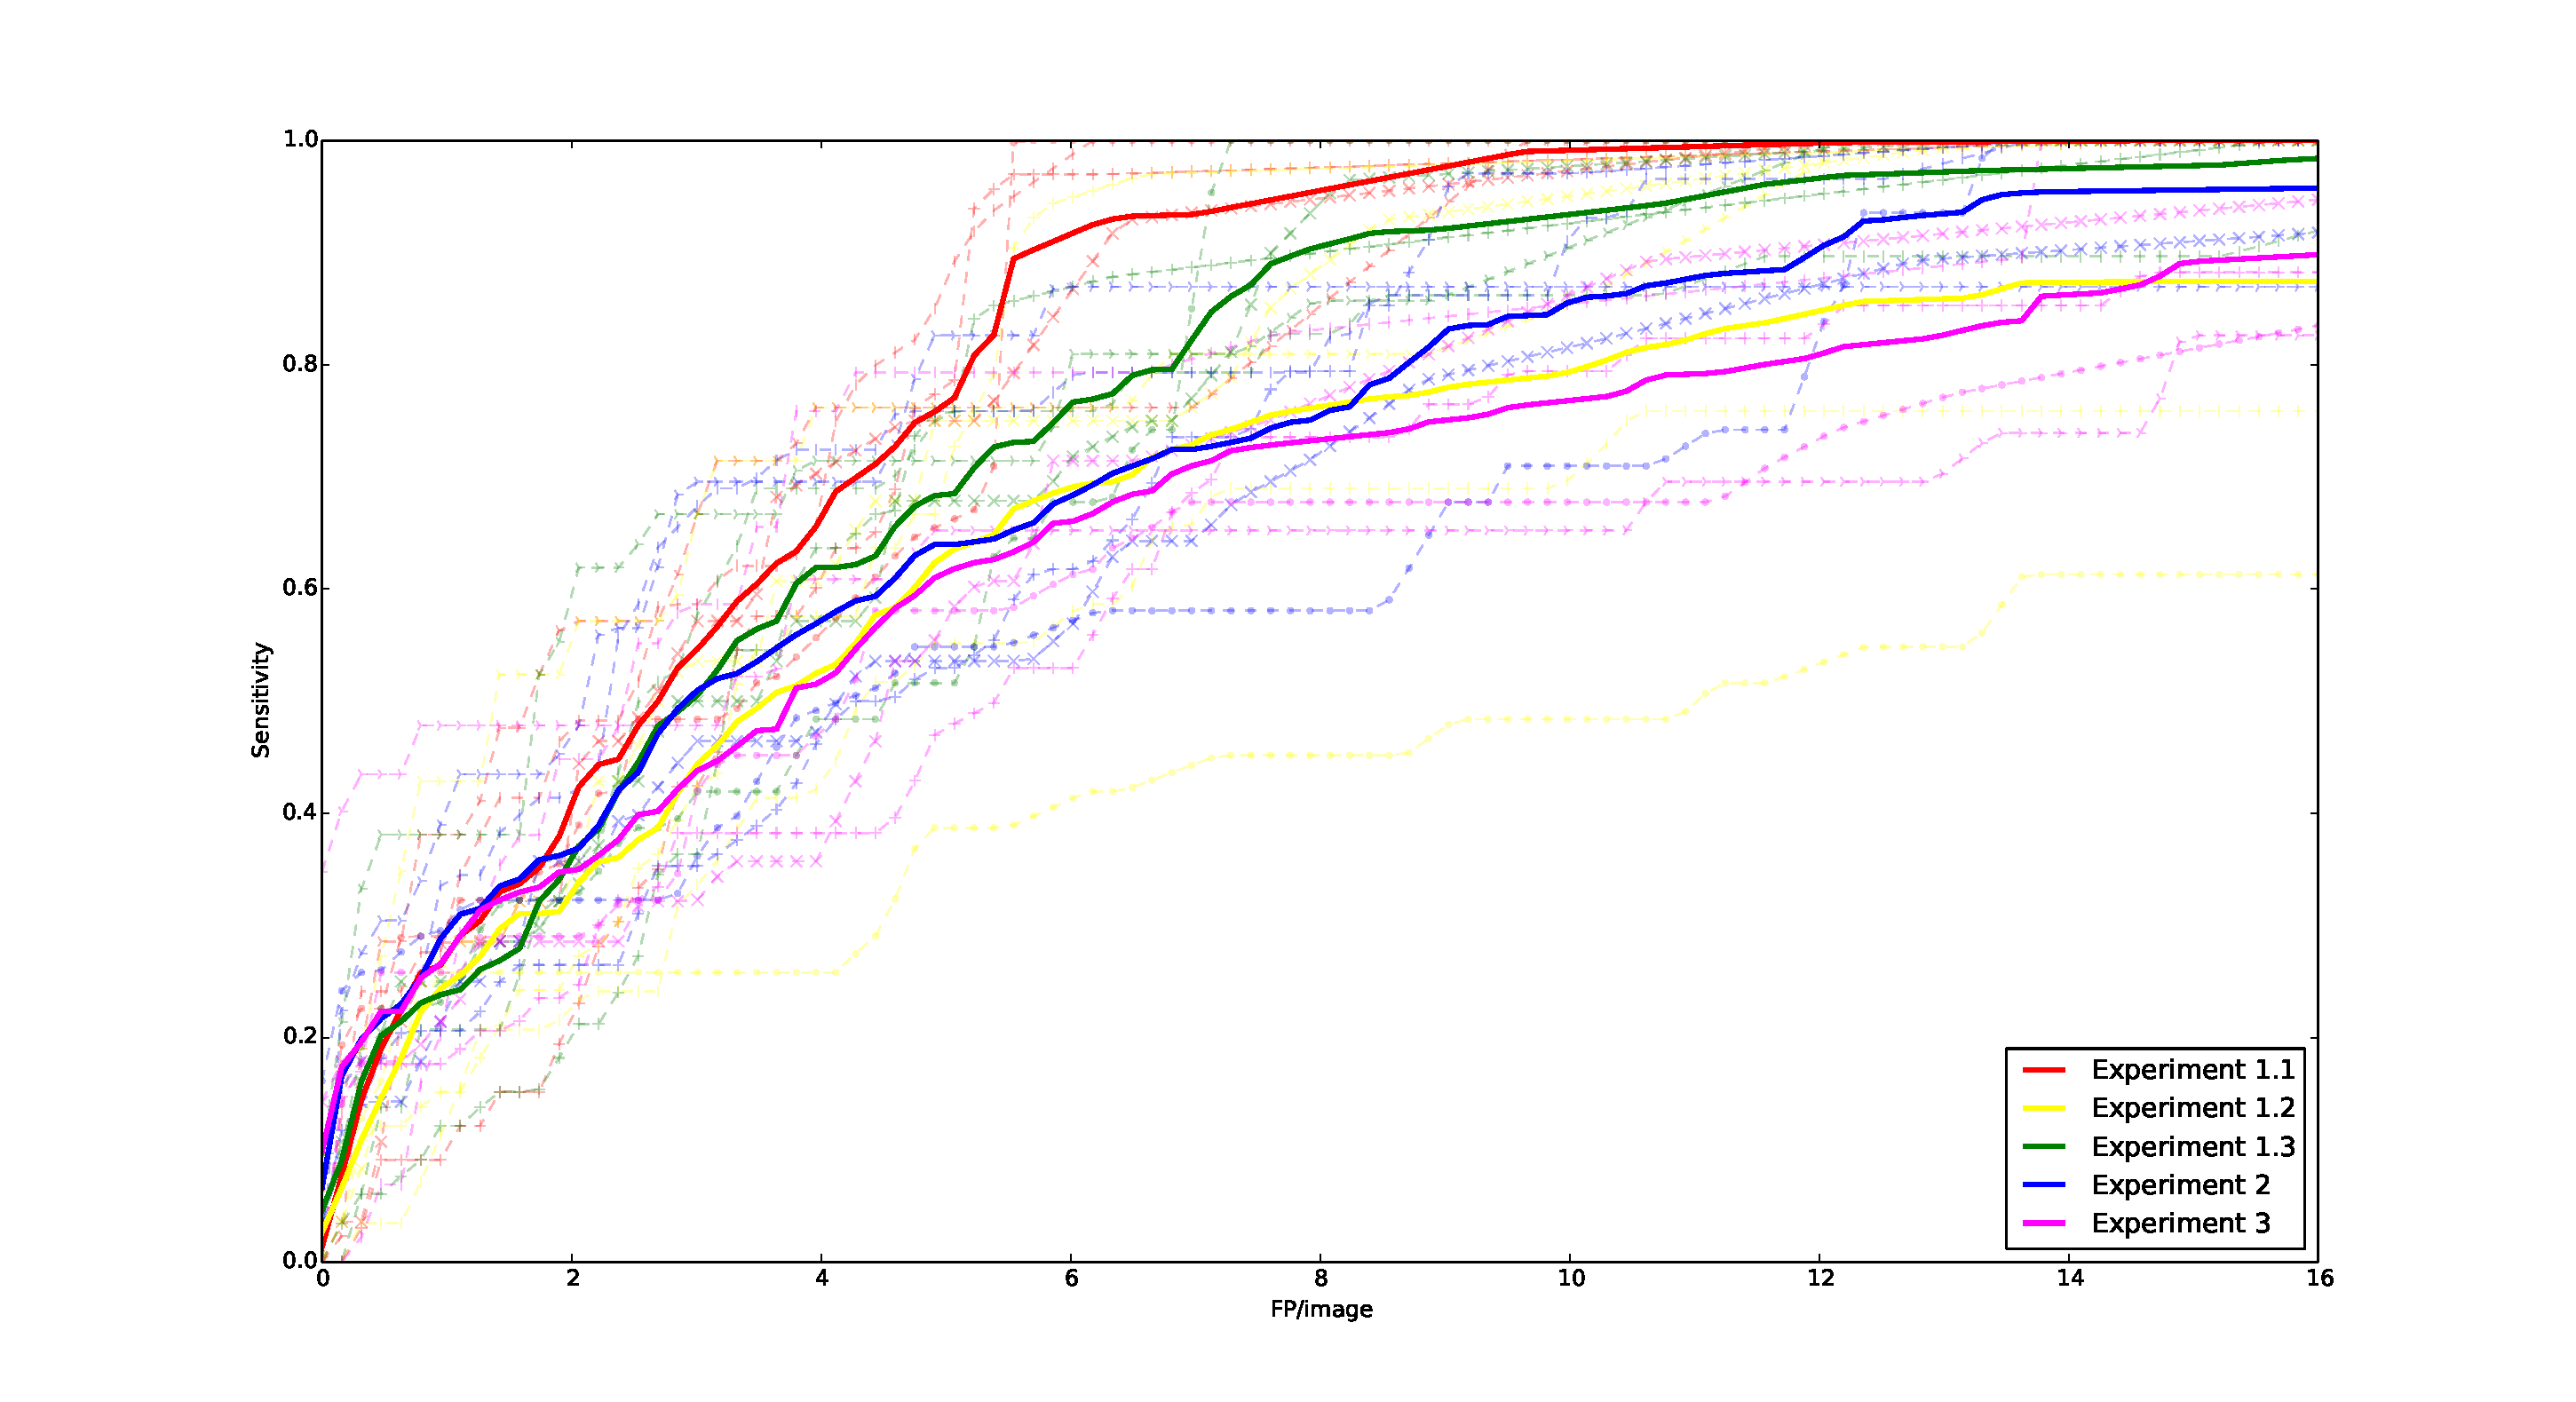
\includegraphics[width=\textwidth]{plots/FROC_curves.pdf}
	\caption[FROC curves]{FROC curves for every experiment and fold. Each experiment appears in a different color. The solid line is the average FROC curve per experiment over all folds. FROC curves ffor each fold are drawn in dashed lines; each fold has a unique marker.}
	\label{fig:FROCResults}
\end{figure}

We can use the sensitivity at a given number of false positives per image to have a single quantitative evaluation of the quality of the model (Tab~\ref{tab:SensitivityResults}).
\begin{table}[h]
	\centering
	\begin{tabular}{l*{6}{c}}
		\hline
		 & \textbf{Fold 1} & \textbf{Fold 2} & \textbf{Fold 3} &\textbf{Fold 4} &\textbf{Fold 5} & \textbf{Average} \\
		\hline 
		Experiment 1.1	&0.09		&\textbf{0.29}	&0.28	&0.29	&0.38	&0.26\\
		Experiment 1.2	&0.15		&0.28		&0.13		&0.26	&0.43	&0.25\\
		Experiment 1.3	&0.12		&0.25		&-			&0.24	&0.38	&-\\
		Experiment 2	&\textbf{0.21} &0.21	&\textbf{0.35}		&\textbf{0.30}	&0.41	&\textbf{0.29}\\
		Experiment 3	&0.18		&0.21		&0.22		&0.26	&\textbf{0.48}	&0.27\\
		\hline
	\end{tabular}
	\caption[Sensitivity at 1 FP/image for the final models]{Sensitivity at 1 FP per image. Best model in each column is shown in bold.}
	\label{tab:SensitivityResults}
\end{table}
% discussion: That there is a lot of variance depending on what fold you are in, this is mostly due to the examples in the test set than those in the training set as those in the training set
% discussion: that x model is usually better
% discussion: Effect on 1 of enhancement and weighted loss.
% discussion: that using a weighted loss usually help converged into a higher range (rather than all being very negative close to zero, now predictions ranged from 0-1)

To get a sense of the qualitative value of our results, we examined the output produced by each network in some chosen examples (Appendix~\ref{app:examples}).


\section{Discussion}
We found that....

\begin{comment}
\section{Summary}
Results for Experiment 1 and Experiment 2 were both equally poor. Experiment 3 produced average results. We believe that it is because of this and this. this could be done... or whatever.
\end{comment}
